\section{\ttt}
\label{sec:treetalker}

To demonstrate the power of the network-side adaption, we decided to adapt a legacy-device which has been in real-world use for some time.
We decided on the ''Treetalker'' platform\footnote{\url{https://www.nature4shop.com/}}, which is a product for distributed tree-health monitoring.
This platform has been in use in many areas in the world for example in Moscow city with 250 TreeTalkers or a cooperation with the Peking University. \footnote{https://www.nature4shop.com/our-vision/}

The platform vendor sells both the sensor-devices (henceforth simply called \textit{Treetalker}), as well as a basestation (henceforth called \textit{TTCloud}), which can be used to aggregate data via LoRa and upload it to a proprietary cloud-storage provider via GSM.
The ''Treetalker''-platform is proprietary, and does not give buyers access to the device firmware.

For our project, we aimed to replace the static \textit{TTCloud}, with a more versatile gateway, to allow for dynamic reconfiguration of all \textit{Treetalkers}.
We call the resulting system \ttt.

The TTCloud, and its associated Treetalkers, can be configured via text-message, also, collected data is sent to the cloud-backend via a mobile data connection\footnote{the operator needs to provide their own SIM-card with a Text-/Data-Plan}

While LoRa-alliance certified hardware provides a dedicated network-layer-protocol, called \textit{LoRa-WAN} which deals with collisions, addressing, and other issues resulting from the shared-medium characteristic of LoRa, the \textit{Treetalker}-vendor decided to forgo this higher-level protocol in favor of using the LoRa-PHY-layer directly.

For this reason, communication with each \textit{Treetalker} needs to be scheduled manually in such a way that avoids collisions.

In order to replace the \textit{TTCloud} with our own gateway, we performed a blackbox-analysis of \textit{Treetalker's} behaviour and network communications, to understand the communication protocol.

Communication between the TTCloud and its sensor-stations is a call-response-protocol, initiated by the TreeTalker.
The TTCloud's command message contains 4 fields, with which the Treetalker's behaviour can be influenced.
\textit{Sleep} is the time that the device will sit idle in between measurements (defaults to 1 hour).
\textit{Heating Time}, that is how long the Treetalker will run its internal heater before taking the second set of heat-probe measurments.
Lastly, we have the \textit{time slot} and \textit{slot length}.
These values govern the time that the device will wait between measurements and sending measurement data, it appears that these two values are simply multiplied to get the time-to-wait before transmitting.

In normal operation, with a vendor-supplied gateway, the sleep- and heat-time are user-configurable, but fixed, and the same for all Treetalkers attached to the gateway.
The time slot length will also be the same for all nodes, while the gateway will assign each Treetalker a unique time slot.
Again, this is necessary due to the vendor's refusal to use the LoRaWAN-protocol, which includes a mechanism for collision-avoidance, but since the Treetalker-system uses the raw \textit{LoRaPHY}-layer, the gateway needs to schedule transmission manually.
For this reason, there is also no way for a Treetalker-network to coexist with other LoRa-networks in the same area, since collisions would be plenty and unrecoverable.

Lastly, when used as intended, the system has no interactivity.
The only way for a user to ''interact'' with the system is by downloading a CSV-file containing the measurement data from the vendor's ''cloud'' backend.

With the insights gathered by our analysis we were able to fully replace and improve the gateway functionality, which allowed us to bring \mm to the treetalker-network.

\subsection{General Design}
\label{sec:treetalker:design}
% System: Alle Treetalker, Ziel: Daten generieen und sie verfügbar machen
% Environment: LoRa Gateway (normalerweise TTCloud) -> Internet
% Mechanism: Lora 
% Interceptor: TTT + Remote (zusammen ForestEdge)
% Unobtrusive: TreeTalker soll keinen Unterschied zw. TTC und ForestEdge erkennen können

Based on the ring-model described in \ref{sec:design}, this scenario contains the following components:
a) The \textit{system}, in this case, is a swarm of deployed Treetalkers in a forest, its goal is the collection of accurate environmental data and to make it available to users.
b) The \textit{environment} starts with the vendor-supplied TTCloud and communicates with the vendors backend to make the aggregated data available for download.
Therefore the TTCloud also contains the required internet up-link.
c) The \textit{mechanism}, which allows the Treetalker swarm to talk to the system, is LoRa.
d) \textit{\ttt} is the \textit{interceptor}.
It replaces the vendor locked TTCloud, communicates with the Treetalker swarm via LoRa, and ultimately allows users to access the data in a more convenient format.
Furthermore, it enhances the functionality of the system as a whole by introducing anomaly detection and therefore improve the quality of the collected data.
e) This approach is \textit{unobtrusive}, since the Treetalkers are unable to distinguish between a first-party TTCloud and \ttt.

%Based on the ring-model described in section \ref{sec:design}, this scenario can be expressed as a 3-ring design.
%The innermost ring, the Treetalker's \textit{firmware} is unaccessible to us, as are the next two, the \textit{hardware} ring and the \textit{link} ring.
%This is all due to the Treetalker-platform being a proprietary black-box, and using an equally closed-source LoRa-module for communication.
%It is therefore only at layer 4, the \textit{network} itself, where we can attach ourselves.
%The particular \mm we are applying, rather than the insertion of an interring, or modification of an existing ring, is the wholesale replacement of this fourth ring with our own hardware.

Our network architecture employs two separate decision making instances, one is located on the physical device in the forest, which communicates directly with the Treetalker swarm, and only has data on its directly connected sensors-nodes.
The second, centralized ''aggregator'' instance on the backend, has global knowledge of all nodes in the network.

When the local decision engine receives a packet, it both stores the data locally and also sends it onwards to the global aggregator, which periodically aggregates all the data from all the nodes and computes relevant benchmark values. 
These are then distributed to all stations.
When it generates a reply packet, the local decision engine performs a statistical evaluation on the node's previous measurement data, and how it relates to the aggregator-supplied benchmark values.
If it detects an anomaly, it may require the Treetalker to rerun its measurements by sending a specially crafted command packet with a short sleep time.

In order to make meaningful decisions, concept recognition is necessary.
This is done by comparing a long-running, and short-running time-window of the data.
It has been shown that the calculation of the twofold standard deviation for short-running windows is already sufficient to be able to make decisions - for example, whether a new measurement is necessary or these new values can be appointed as the new standard.
In general, the preferred decision is to reduce the upcoming measurement interval in order to verify and increase the accuracy of the collected data.
Due to the minor costs on battery and data transmission over Lora, even a 20\% increase in measurements is insignificant for the overall energy consumption. 

\subsection{Evaluation}
\label{sec:treetalker:evaluation}

\subsubsection{Response Time}
\label{sec:evaluation:response-time}

The protocol employed by the Treetalker is a simple two-way exchange of data, where the treetalker will send measurements to the associated cloud and wait for new configuration parameters.
If it does not receive a response to its data packet after a certain time, it assumes that the cloud is offline and falls back to repeating the message ad-infinitum.
Thus,in order to be a viable alternative to the first-party TTCloud, the \ttt needs to be able to respond to each received data-packet within reasonable time.

In order to compare the response time of our system versus the TTCloud, we used a test-setup of a single Treetalker, in combination with a passive sniffing node, which recorded all LoRa-traffic.

\begin{figure}
    \centering
    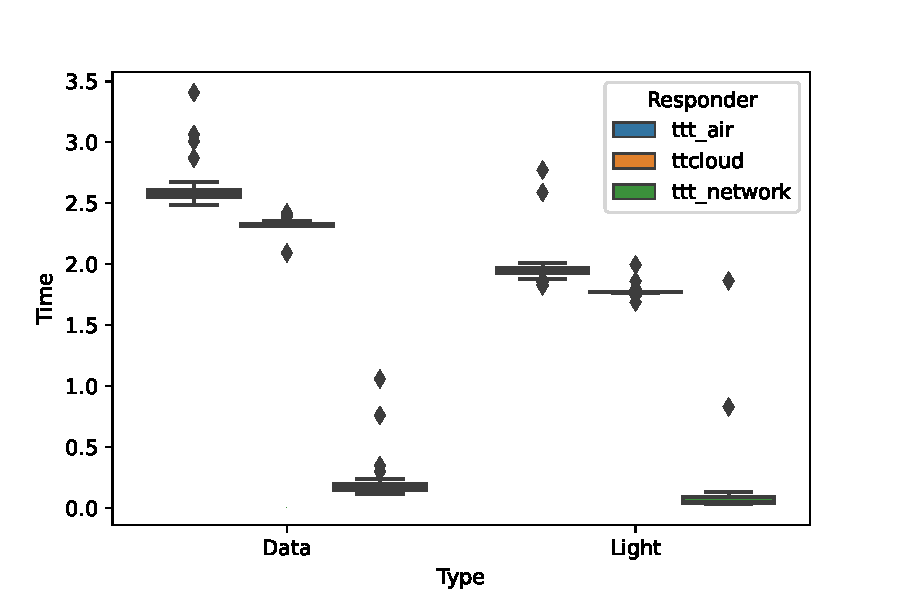
\includegraphics[width=\linewidth]{figures/response_times.pdf}
    \caption{Response time of both the first-party \textit{TTCLoud}, as well as \textit{\ttt}.}
    \label{fig:evaluation:ttt_response}
\end{figure}

As can be seen in figure \ref{fig:evaluation:ttt_response}, the \ttt is capable delivering responses with a similar delay as the TTCloud.
The three bars are, from left to right: 1) The total response time of \ttt, including both the time it takes to generate a reply packet, as well as transmitting it via LoRa. 2) The response time of the first-party TTCloud, also including LoRa Transmission. 3) The time it takes \ttt just to generate the reply packet.
In fact, the actual time it takes to arrive at a decision and craft the reply-package is less than one quarter of the total time, the other three quarters being the time necessary to transmit the packet via LoRa.
The TTCloud, which does no further processing whatsoever, does have the advantage of only sending the same reply every time, thus not requireing any additional time for computations of any kind.
Therefore, it is sometime very slightly faster, though not by any significant margin.

While there are occasional outliers, wherein the analysis of a packet and the generation of the appropriate response packet take significantly longer, these are very rare, being 4 out of 200 cases.
This is most likely due to database-queries occasionally taking longer, probably due to scheduling issues.

\subsubsection{Anomaly Detection}
\label{sec:evaluation:anomaly-detection}

To evaluate whether the anomaly-detection functions as intended, we drew upon real-world data gathered by a Treetalker-deployment, which was created as part of the \textit{Nature 4.0} project of the University of Marburg.
This deployment is comprised of 100 Treetalker which were set up in a university-owned parcel of forest and has been continually gathering sensor data for the past 2 years.

The evaluation was performed by injecting historical data into the policy-engine in chronological order, thus simulating a replay of the 2 year data-gathering-process.

\begin{table}[tb]
    \centering
    \caption{Anomalous and critical events found in historical data}
    \label{tab:evaluation:anomalies}
    \begin{tabular}{lcccc}
        \toprule
        Type & Position & Movement & Stem Temp. & Air Temp.  \\ \midrule
        Anomalous & 2182 & 108 & 443 & 0 \\
        Critical & 6313 & 105 & 183 & 1 \\
        \bottomrule
    \end{tabular}
\end{table}

As becomes obvious from table \ref{tab:evaluation:anomalies}, the vast majority of events are produced by the accelerometer, and more specifically by the values denoting the sensor's position.

Further investigation of the data revealed that this seems to be due to a systematical fault in either the installed sensor itself, or the method in which this sensor is queried by the onboard electronics.
The data reported by the Treetalker for this sensor seems to be completely erratic and entirely unsuited as a basis for further decision-making.
This fault had previously not been noticed by the operator and could have wrought havoc on data analysis performed on the gathered data, but with the aid of \ttt, we were able discover this deficiency before it could impact further decision-making.

In conclusion, by applying our interception-concept to the Treetalker-network, we were able to significantly improve the system's functionality and performance.
We were also able to leverage behavioral modification to enable interactivity on an otherwise static system, which allowed us to recognise faulty sensors and prevent corrupted data from derailing other research projects.
